\documentclass[a4paper]{article}

%% Language and font encodings
\usepackage{polski}
\usepackage[polish]{babel}
\usepackage[utf8x]{inputenc}
\usepackage[T1]{fontenc}
\usepackage{pdfpages}
\usepackage{indentfirst}
\usepackage{listings}
\usepackage{isotope}

\usepackage{csvsimple}
\setlength{\tabcolsep}{2pt}

% Adjust penalties
\brokenpenalty=1000
\clubpenalty=1000
\widowpenalty=1000

% Don't break in math expressions
\relpenalty=10000
\binoppenalty=10000

%% Sets page size and margins
\usepackage[a4paper]{geometry}

%% Useful packages
\usepackage{amsmath}
\usepackage{graphicx}
\usepackage[colorlinks=true, allcolors=blue]{hyperref}
\usepackage{booktabs}
\usepackage{cancel}
\usepackage{tikz}

\usepackage{float}

\renewcommand\thesection{\arabic{section}.}
\renewcommand\thesubsection{\arabic{section}.\arabic{subsection}.}
\renewcommand\thesubsubsection{\arabic{section}.\arabic{subsection}.\arabic{subsubsection}.}

% The following commands are not supported in PSTricks at present
% We define them conditionally, so when they are implemented,
% this pgf file will use them.
\ifx\du\undefined
  \newlength{\du}
\fi
\setlength{\du}{15\unitlength}

\newcommand{\Vsp}[1]{\vtop to #1 {}}
\newcommand{\Hsp}[1]{\hbox to #1 {}}
\newcommand{\Small}{\scriptsize}

\title{Sprawozdanie nr 8}
\date{}


\begin{document}

\begin{center}
\begin{tabular}{|p{5.5cm}|l|l|c|}
    \hline
	% Row 1.1  
	    Wydział \Vsp{4mm} &
	    \multicolumn{1}{|l}{Dzień} &
	    poniedziałek $17^{15} - 19^{30}$ &
	    Nr zespołu \\
	% Row 1.2
	    \mbox{\small{Matematyki i Nauk Informatycznych}} &
	    \multicolumn{1}{|l}{Data}  &
	    &
	    \multicolumn{1}{c|}{\Large{18}} \\
    
    \hline
	% Row 2.1 
	    Nazwisko i Imię: &
	    \Small Ocena z przygotowania &
	    \Small Ocena ze sprawozdania &
	    \Small Ocena Końcowa \\
	% Rows 2.2-2.4
	    1. Jasiński Bartosz & & &\\
	    2. Sadłocha Adrian & & & \\
	    3. Wódkiewicz Andrzej & & & \\

    \hline
    % Row 3.1
	    \multicolumn{2}{|l|}{Prowadzący \Vsp{4mm}} &
	    \multicolumn{2}{|l|}{Podpis prowadzącego} \\  
    % Row 3.2
    	\multicolumn{2}{|l|}{dr hab. Jacek Gosk} &
    	\multicolumn{2}{|l|}{} \\    	
    \hline
\end{tabular}
\label{pieczatka}
\end{center}

{\let\newpage\relax\maketitle}
\setcounter{secnumdepth}{2}


\section{Opis ćwiczenia i wstęp teoretyczny}

Celem ćwiczenia było zapoznanie się z działaniem lampy elektronowej, wykazanie zależności 
natężenia prądu anodowego diody od napięcia przyłożonego na diodę oraz wyznaczenie temperatury katody
na podstawie wykonanych pomiarów.

Przed rozpoczęciem ćwiczenia, w sali laboratoryjnej przygotowany został uprzednio układ pomiarowy,
którego schemat przedstawiono na rysunku \ref{schemat}.

% \begin{figure}
% \centering
% 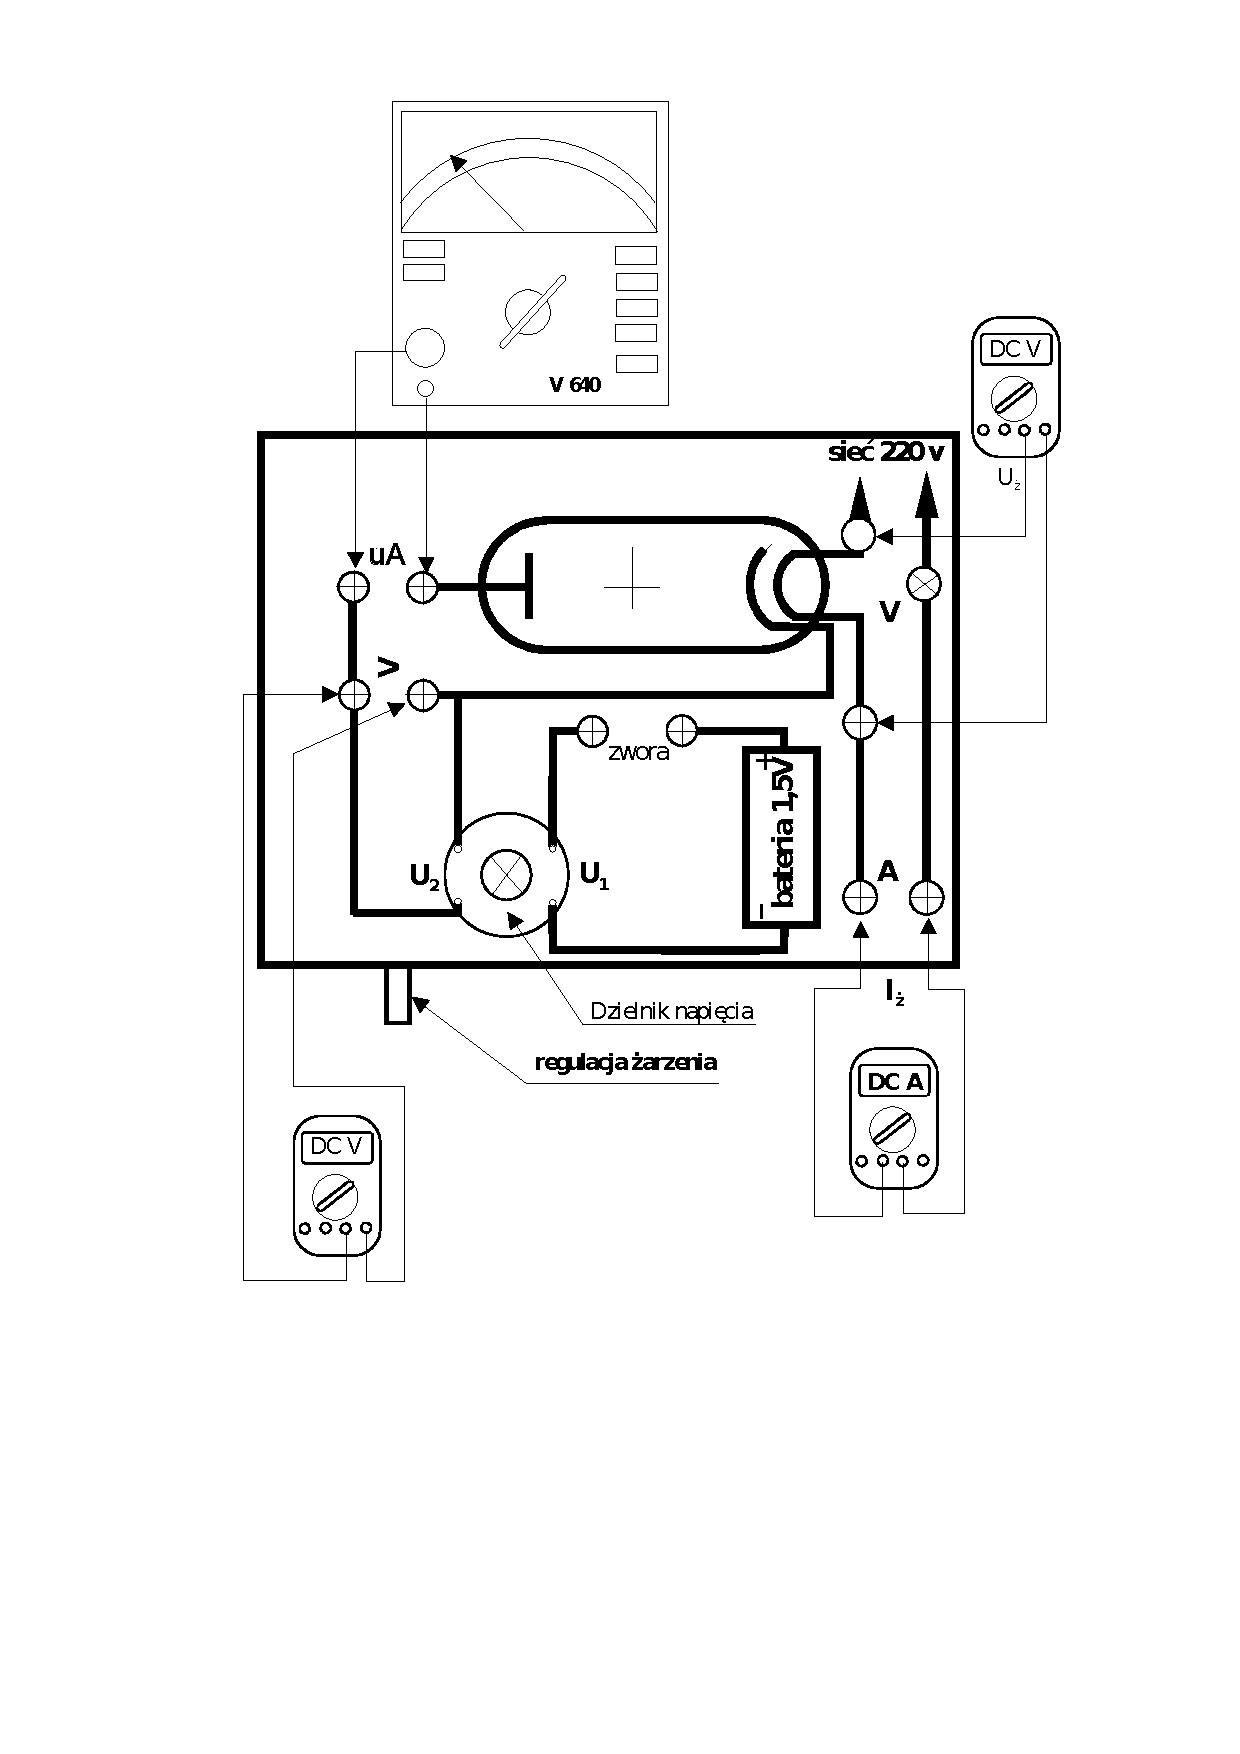
\includegraphics[scale=0.5]{schemat.png}
% \caption{Schemat układu pomiarowego}
% \label{schemat}
% \end{figure}

Układ został przygotowany w taki sposób, aby napięcie przyłożone do lampy elektronowej hamowało
ruch elektronów opuszczających katodę (biegun dodatni baterii połączony został z katodą, a ujemny z anodą).
Budowa układu pozwalała jedynie na regulowanie wartości napięcia \textit{w jedną stronę}.
Z powodu braku możliwości zamiany polaryzacji przykładanego napięcia, nie można było wyznaczyć 
w ćwiczeniu wartości napięcia kontaktowego między okładkami.

Korzystaliśmy z przybliżenia, że elektrony wewnątrz lampy można opisać jako gaz elektronów, oraz dalej, 
z powodu znajdowania się ich w próżni nie występują oddziaływania między nimi -- jako gaz doskonały.
Były to podstawy do założenia, że prędkości elektronów przemieszczających się w kierunku anody 
mają rozkład Maxwella.

Wzór, który uwzględnia ten rozkład i posłużył w ćwiczeniu za podstawę opracowywania wyników pomiarów,
opisuje zależność między natężeniem prądu anodowego a napięciem przyłożonym do lampy.

\begin{align}
	I_a(U_a; T) = I_{a_0} \exp{\left(-\frac{e U_a}{k T}\right)}
\label{eq1}
\end{align}

gdzie $I_a$ to natężenie prądu anodowego, $U_a$ to zmienna niezależna będąca napięciem przyłożonym do lampy,
$T$ to parametr równania, będący temperaturą katody, zaś pozostałe czynniki to następujące stałe:
\begin{itemize}
\item $I_a$ -- prąd \textit{początkowy}
\item $e$ -- ładunek elementrarny z minusem
\item $k$ -- stała Boltzmanna
\end{itemize}

Analizując równanie, mozna stwierdzić, że $I_{a_0}$ to \textit{zerowe} natężenie prądu anodowego przy
braku przyłożonego dodatkowego napięcia ($U_a = 0 \text{V}$). Ponieważ napięcie $U_a$ jest hamujące,
dlatego przyjmuje w naszych rozważaniach wyłącznie wartości ujemne, stąd (pamiętając o ujemnej wartości
ładunku $e$) argument funkcji wykładniczej ma wartość ujemną. Zatem mierzona wartość $I_a$ powinna 
znajdować się w przedziale $(0; I_{a_0}]$ i maleć wraz ze zwiększaniem wartości bezwzględnej
napięcia hamującego. Dodatkowo, wraz ze zwiększaniem temperatury $T$ wykres funkcji wykładniczej
\textit{oddala} się w przedziale $(-\infty; 0)$ od osi $OX$, co wpływa na zwiększenie wartości funkcji
$I_a$ dla ustalonego $x$.

Do dalszego opracowywania wyników wyprowadzono drugi wzór ze wzoru \ref{eq1}, logarytmując równanie
stronami:

\begin{align}
	\ln{\frac{I_a}{I_{a_0}}} = -\frac{e U_a}{k T}
\label{eq2}
\end{align}

Poszukiwana była zależność liniowa, gdzie:
\begin{itemize}
\item $X = U_a$ -- zmienna niezależna
\item $Y = \ln \frac{I_a}{I_{a_0}}$ -- zmienna zależna
\item $a = -\frac{e}{kT}$ -- współczynnik kierunkowy
\end{itemize}





\section{Pomiary i opracowanie wyników}
W naszym doświadczeniu dostaliśmy gotową diodę próżniową oraz mierniki natężenia oraz napięcia, na początku ćwiczenia zmonotowaliśmy obwód w sposób widoczny na rysunku \ref{schemat}. Ustawiliśmy prąd żarzenia na $0.375 A$ przy pierwszym pomiarze oraz $0.385 A$ przy drugim. Połączyliśmy katodę z anodą przez mikroamperomierz. Zanim włączyliśmy żarnik prąd wskazywany na mikroaperomierzu wynosił 0A. Po ogrzaniu katody po pewnym czasie prąd ustabilizował się na 0.383 µA. Zauważyliśmy następującą prawidłowość, jeśli temperatura żarnika rosła wówczas prąd w obwodzie żarnika malał (z powodu wzrostu oporu wraz ze wzrostem temperatury). W tym samym czasie prąd anodowy rosnął wraz z rozgrzewaniem lampy elektronowej.\\
Po zwarciu oporu na baterii dołączyliśmy woltomierz do obwodu mierzący napięcie na anodzie. Podawaliśmy ujemne napięcie na anodę za pomocą dzielnika napięcia, wtedy prąd anodowy zaczął maleć.
\\ \textbf{Rozkład Maxwella} określa on rozkład prędkości cząstek gazu doskonałego. Określa on liczbę cząstek które w jednostce obiętości mają prędkości z przedziału $<v, v + dv>$. W naszym doświadczeniu wyemitowane elektrony możemy traktować właśnie jako cząstki gazu doskonałego, ponieważ są one emitowane z gęstością o 10-15 rzędów mniejszą niż w metalu, dzięki temu nie oddziaływują ze sobą. 


\begin{figure}[h!]
\centering
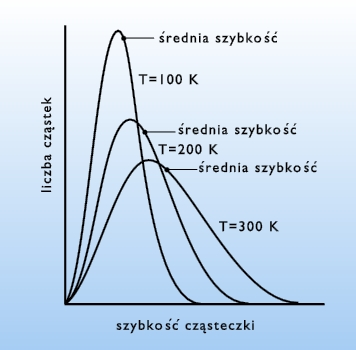
\includegraphics[scale=0.5]{rozlad_maxwella.jpg}
\caption{Rozkład Maxwella \url{zasoby1.open.agh.edu.pl/dydaktyka/2_stany_skupienia/02_02_46.jpg}}
\end{figure}

\newpage
\subsection{Pierwszy pomiar}
Wyniki pomiarów wykonanych i niepewności dla pierwszego prądu żarzenia są zawarte w tabeli \ref{T1_pomiar}. Niepewność pomiarowa natężenia prądu wyraża się wzorem: 
\begin{align*}
u_{I_{a}} = \sqrt{(\frac{\Delta I}{\sqrt{3}})^2 + (\frac{\Delta I_{E}}{\sqrt{3}})^2}
\end{align*}
gdzie:\\
$u_{I_{a}}$ - niepewność pomiaru wartości natężenia \\
$\Delta I$ - niepewność amperomierza \\
$\Delta I_{E}$ - niepewność eksperymentatora\\

W naszym przypadku amperomierz był wychyłowy i posiadał pierwszą klasę czyli by wyznaczyć $\Delta I$ posłużyliśmy się wzorem:
\begin{align*}
\Delta I = klasa\ urządzenia * \frac{zakres}{100} = 0.0015
\end{align*}
podanym na wykładzie wstępnym.
Przyjeliśmy że niepewność eksperymentatora jest równa $\frac{1}{2}$ najmniejszej podziałki.\\

Wyniki znajdujące się w kolumnie $u_{U}$ są niepewnościami pomiarowymi napięcia prądu. Wartość niepewności zależy zarówno od jakości urządzenia pomiarowego jak i samego odczytu, w naszym przypadku wyraża się wzorem:
\begin{align*}
u_{U} = \frac{0,3 \% \cdot rdg + 1 \cdot dgt}{\sqrt{3}}
\end{align*}
gdzie: \\
$rdg$ - zmierzona wartość \\
$dgt$ - dokładność pomiaru \\

Wyniki dla niepewności wyznaczenia logarytmu stosunku prądu zmierzonego do prądu początkowego obliczyliśmy z następujacego wzoru:
\begin{align*}
u_{ln} = \sqrt{(\frac{1}{I_{a}})^2 \cdot U_{I_{a}}^2 + (- \frac{1}{I_{a0}})^2 \cdot U_{I_{a0}}^2 }
\end{align*}
gdzie:\\
$u_{ln}$ - niepewność logarytmu stosunku wartości natężenia zmierzonego do prądu początkowego \\
$I_{a}$ - wartość zmierzonego prądu\\
$I_{a0}$ - wartość prądu początkowego\\
$u_{I_{a}}$ - niepewność pomiaru wartości natężenia \\
$u_{I_{a0}}$ - niepewność pomiaru wartości natężenia początkowego \\

W większości punktów na wykresie nie jest widoczna niepewność, ponieważ są one mniejsze od punktów którymi są zaznaczone pomiary.


\begin{table}[h!]
\centering
 \begin{tabular}{ | l | l | l | l | l | l | l | l | }
 \hline
L.p & U[V] & $I_{a}$ [µA] & $U_{I_{a}}$ [µA] & $U_{U}$ [V] & $ln(l_{a}/l_{a0})$ & $U_{ln}$ & $\sqrt(U)$ \\ \hline
1 & 0.000 & 0.135 & 0.0017 & 0.00058 & 0.0000 & 0.0178 & 0.0000 \\ \hline
2 & -0.012 & 0.110 & 0.0017 & 0.0006 & -0.2048 & 0.0199 & 0.1095 \\ \hline
3 & -0.018 & 0.105 & 0.0017 & 0.00061 & -0.2513 & 0.0205 & 0.1342 \\ \hline
4 & -0.021 & 0.100 & 0.0017 & 0.00061 & -0.3001 & 0.0212 & 0.1449 \\ \hline
5 & -0.030 & 0.090 & 0.0017 & 0.00063 & -0.4055 & 0.0227 & 0.1732 \\ \hline
6 & -0.038 & 0.080 & 0.0017 & 0.00064 & -0.5232 & 0.0247 & 0.1949 \\ \hline
7 & -0.045 & 0.070 & 0.0017 & 0.00066 & -0.6568 & 0.0274 & 0.2121 \\ \hline
8 & -0.055 & 0.065 & 0.0017 & 0.00067 & -0.7309 & 0.0290 & 0.2345 \\ \hline
9 & -0.065 & 0.055 & 0.0017 & 0.00069 & -0.8979 & 0.0334 & 0.2550 \\ \hline
10 & -0.075 & 0.050 & 0.0017 & 0.00071 & -0.9933 & 0.0363 & 0.2739 \\ \hline
11 & -0.089 & 0.040 & 0.0017 & 0.00073 & -1.2164 & 0.0443 & 0.2983 \\ \hline
12 & -0.097 & 0.035 & 0.0017 & 0.00075 & -1.3499 & 0.0502 & 0.3114 \\ \hline
13 & -0.107 & 0.030 & 0.0017 & 0.00076 & -1.5041 & 0.0580 & 0.3271 \\ \hline
 \end{tabular}
\caption{Wyniki wielokrotnych pomiarów i niepwności dla pomiaru pierwszego}
\label{T1_pomiar}
\end{table}




\begin{figure}[h!]
	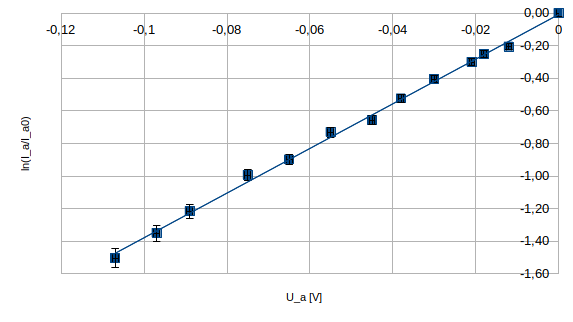
\includegraphics[scale=1]{T1_ln_U}
	\centering
	\caption{Wykres zależności logarytmu stosunku zmierzonego natężenia do natężenia początkowego od napięcia. Pomiar pierwszy}
\end{figure}

Używając metody najmniejszych kwadratów policzyliśmy temeperaturę katody wysyłającej elektrony. Współczynnik kierunkowy prostej wynosi:
\begin{align*}
a \approx 13.81 (0.11)
\end{align*}

Z tego otrzymujemy temperaturę katody oraz błąd:
\begin{align*}
T = \frac{e}{k \cdot a} \approx 840.36 K
\end{align*}

\begin{align*}
u_{T} = \sqrt{(\frac{e}{k \cdot a^2}) \cdot u_{a}^2} \approx 6.57 K
\end{align*}


\begin{figure}[h!]
	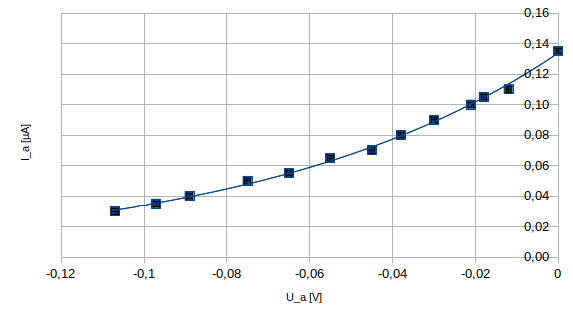
\includegraphics[scale=1]{T1_Ia_U}
	\centering
	\caption{Wykres zależności natężenia od napięcia. Pomiar pierwszy}
\end{figure}

\begin{figure}[h!]
	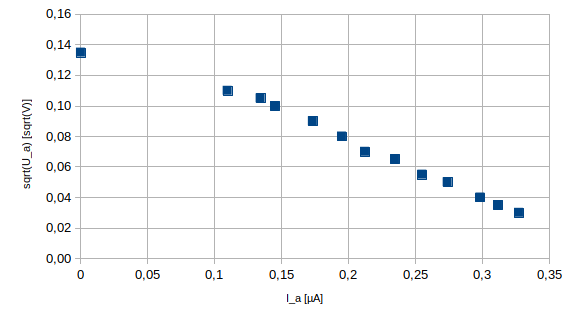
\includegraphics[scale=1]{T1_Ia_sqrtU}
	\centering
	\caption{Wykres zależności natężenia od pierwiastka napięcia. Pomiar pierwszy}
\end{figure}

\newpage
\subsection{Drugi pomiar}
W drugim pomierze w przeciwieństwie do pierwszego zmienialiśmy zakres pomiarów na amperomierzu (z tego wynikają większe niepewności pomiarowe dla 3 pierwszych pomiarów). Analogicznie do poprzedniego pomiaru wyznaczyliśmy tempraturę metodą najmniejszych kwadratów. Współczynnik kierunkowy prostej wynosi:
\begin{align*}
a \approx 12.80 (0.06)
\end{align*}

Z tego otrzymujemy temperaturę katody oraz błąd:
\begin{align*}
T \approx 906.31 K
\end{align*}

\begin{align*}
u_{T} = 3.96 K
\end{align*}



\begin{table}[h!]
\centering
 \begin{tabular}{ | l | l | l | l | l | l | l | l | }
 \hline
L.p & U[V] & $I_{a}$ [µA] & $U_{I_{a}}$ [µA] & $U_{U}$ [V] & $ln(l_{a}/l_{a0})$ & $U_{ln}$ & $\sqrt(U)$ \\ \hline
1 & 0.000 & 0.250 & 0.0168 & 0.00058 & 0.00000 & 0.09522 & 0.00000 \\ \hline
2 & -0.016 & 0.200 & 0.0168 & 0.00061 & -0.22314 & 0.10778 & 0.12649 \\ \hline
3 & -0.038 & 0.150 & 0.0168 & 0.00064 & -0.51083 & 0.13087 & 0.19494 \\ \hline
4 & -0.041 & 0.150 & 0.0017 & 0.00065 & -0.51083 & 0.06826 & 0.20248 \\ \hline
5 & -0.047 & 0.140 & 0.0017 & 0.00066 & -0.57982 & 0.0684 & 0.21679 \\ \hline
6 & -0.055 & 0.125 & 0.0017 & 0.00067 & -0.69315 & 0.06866 & 0.23452 \\ \hline
7 & -0.058 & 0.120 & 0.0017 & 0.00068 & -0.73397 & 0.06878 & 0.24083 \\ \hline
8 & -0.069 & 0.105 & 0.0017 & 0.00070 & -0.8675 & 0.06921 & 0.26268 \\ \hline
9 & -0.085 & 0.085 & 0.0017 & 0.00072 & -1.07881 & 0.07018 & 0.29155 \\ \hline
10 & -0.100 & 0.070 & 0.0017 & 0.00075 & -1.27297 & 0.0715 & 0.31623 \\ \hline
11 & -0.112 & 0.060 & 0.0017 & 0.00077 & -1.42712 & 0.07294 & 0.33466 \\ \hline
12 & -0.125 & 0.050 & 0.0017 & 0.00079 & -1.60944 & 0.07528 & 0.35355 \\ \hline
13 & -0.141 & 0.040 & 0.0017 & 0.00082 & -1.83258 & 0.07940 & 0.37550 \\ \hline
 \end{tabular}
\caption{Wyniki wielokrotnych pomiarów i niepwności dla pomiaru drugiego}
\end{table}

\begin{figure}[h!]
	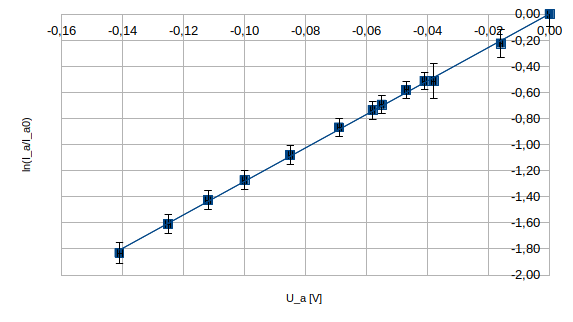
\includegraphics[scale=1]{T2_ln_U}
	\centering
	\caption{Wykres zależności logarytmu stosunku zmierzonego natężenia do natężenia początkowego od napięcia. Pomiar drugi}
\end{figure}

\begin{figure}[h!]
	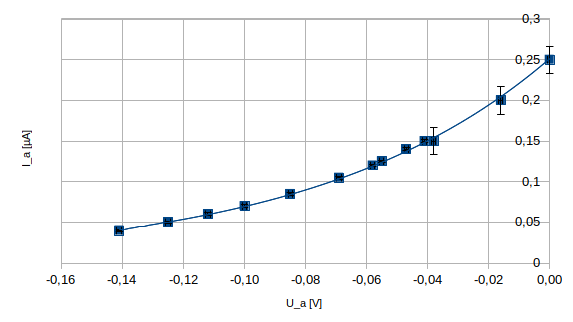
\includegraphics[scale=1]{T2_Ia_U}
	\centering
	\caption{Wykres zależności natężenia od napięcia. Pomiar drugi}
\end{figure}

\begin{figure}[h!]
	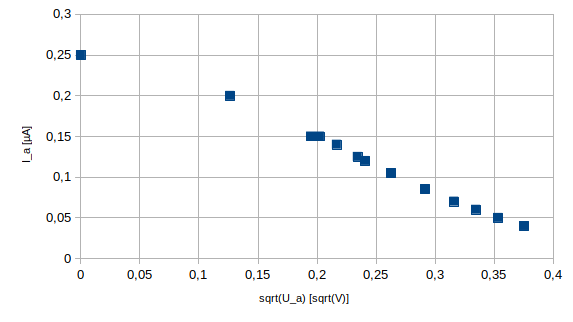
\includegraphics[scale=1]{T2_Ia_sqrtU}
	\centering
	\caption{Wykres zależności natężenia od pierwiastka napięcia. Pomiar drugi}
\end{figure}

\end{document}
